\documentclass{article}

\usepackage{graphicx}
\usepackage{tikz}
\usepackage{tikzsymbols}
\usetikzlibrary{calc,patterns,shapes.geometric}
\pagestyle{empty}
\usepackage[margin=0pt]{geometry}
\geometry{papersize={14in,12in}}

\def\centerarc[#1](#2)(#3:#4:#5){\draw[#1] ($(#2)+({#5*cos(#3)},{#5*sin(#3)})$) arc (#3:#4:#5);}

\begin{document}
	\begin{figure}
		\centering
		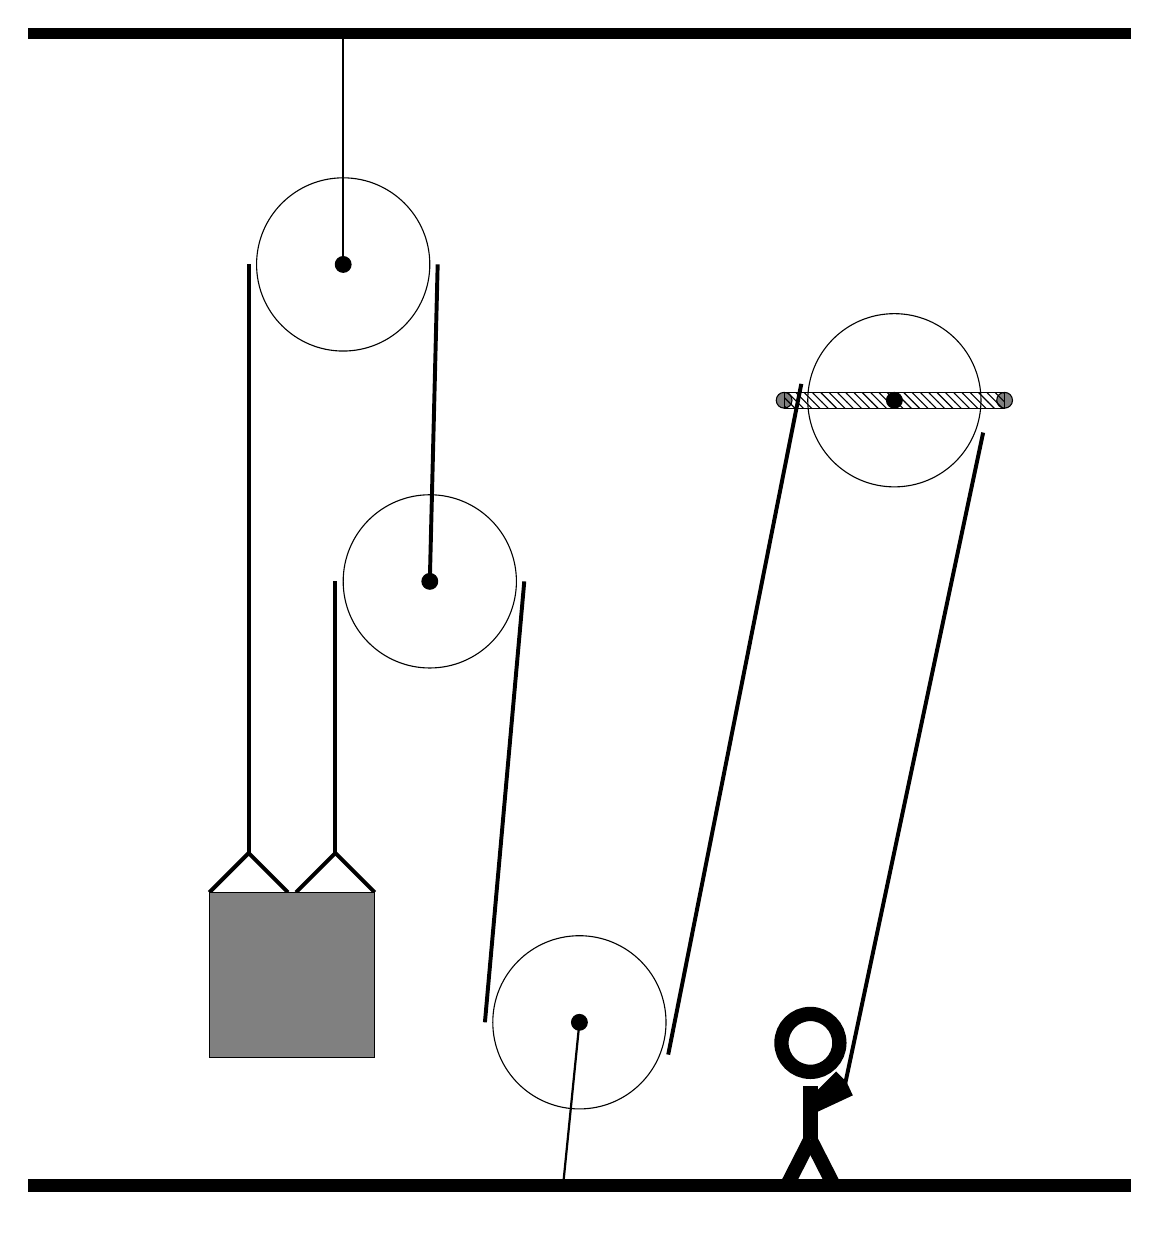
\begin{tikzpicture}
			%%%%% START %%%%%
			\draw[fill=black] (-2, 11.5) rectangle (12, 11.625);
			
			\draw (2, 8.625) circle (1.1);
			\draw[fill=black] (2, 8.625) circle (0.1);
			\draw[thick] (2, 8.625) -- (2, 11.5);
			
			\draw (3.1, 4.6) circle (1.1);
			\draw[fill=black] (3.1, 4.6) circle (0.1);
			
			\draw (5, -1) circle (1.1);
			\draw[fill=black] (5, -1) circle (0.1);
			\draw[thick] (5, -1) -- (4.8, -3);
			
			\draw (9, 6.9) circle (1.1);
			\draw[fill=black] (9, 6.9) circle (0.1);
			\draw[fill=black!50] (7.6, 6.9) circle (0.1);
			\draw[fill=black!50] (10.4, 6.9) circle (0.1);
			\draw[pattern=north west lines, pattern color=black] (7.6, 7.0) rectangle (10.4, 6.8);
			
			\draw[line width = 0.5mm]  (0.3, 0.65) -- (0.8, 1.15) -- (1.3, 0.65);
			\draw[line width = 0.5mm]  (1.4, 0.65) -- (1.9, 1.15) -- (2.4, 0.65);
			\draw[fill=black!50] (0.3, 0.65) rectangle (2.4, -1.45);
			
			\draw[line width = 0.5mm] (0.8, 8.625) -- (0.8, 1.15);
			\centerarc[line width = 0.5mm](2, 8.625)(0:180:1.2000000000000002);
			\draw[line width = 0.5mm] (3.2, 8.625) -- (3.1, 4.6);
			\draw[line width = 0.5mm] (1.9, 4.6) -- (1.9, 1.15);
			\centerarc[line width = 0.5mm](3.1, 4.6)(0:180:1.2000000000000002);
			\draw[line width = 0.5mm] (4.3, 4.6) -- (3.8, -1);
			\centerarc[line width = 0.5mm](5, -1)(180:340:1.2000000000000002);
			\draw[line width=0.5mm](6.1276, -1.4104) -- (7.8182, 7.1083);
			\centerarc[line width = 0.5mm](9, 6.9)(-20:170:1.2000000000000002);
			\draw[line width=0.5mm](10.1276, 6.4896) --  (8.35, -1.9);
			
			\node at (8, -2) {\Strichmaxerl[10][225][25]};
			
			\draw[fill=black] (-2, -3) rectangle (12, -3.15);
			%%%%% END %%%%%
		\end{tikzpicture}
	\end{figure}	
\end{document}